\section{Implementation}
We implemented our analyses for the ES\&S iVotronic voting terminals and we built a web application in order for election officials and advocacy groups to have easy access to our analyses.  Our tool requires the user to upload an event log and a ballot images file; we strongly suggest that they also submit the system log to take advantage of the full range of analyses our tool provides.  The following describes how our tool works.  

\begin{enumerate}
\item
The election is performed on DRE machines; Figure~\ref{fig:subfig1} shows the ES\&S iVotronic voting machine.  Event logs, ballot images files, and system logs are produced after each election.
\item
Election officials upload these files to AuditBear.  This web application is found at www.audit-bear.org, as displayed in Figure~\ref{fig:subfig2}.  
\item
AuditBear produces reports.  Figure~\ref{fig:subfig3} is an example of one such report, titled \textquotedblleft PEBs Not Uploaded.\textquotedblright
\item
Election officials are warned about possible miscounts or procedural errors. 
\end{enumerate}

\begin{figure}[h]
\centering
\mbox{
\subfigure[iVotronic Machine]{
	\epsfig{figure=machine.png,width=1in}
	\label{fig:subfig1}}
\subfigure[audit-bear.org]{
	\epsfig{figure=indexpage.png,width=1in}
	\label{fig:subfig2}}
\subfigure[Reports]{
	\epsfig{figure=report2.png,width=1in}
	\label{fig:subfig3}}}
\caption{Workflow of AuditBear}
\label{auditBear}
\end{figure}



%\begin{figure}
%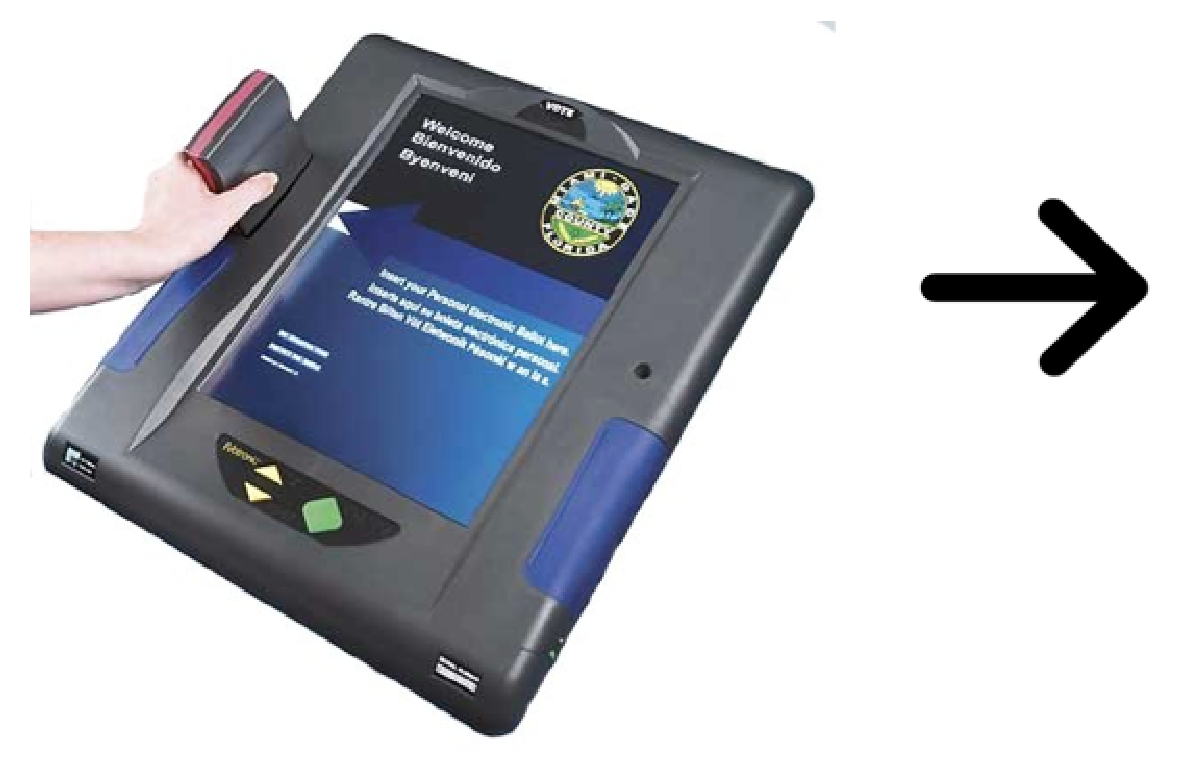
\includegraphics[scale=0.10]{machine.eps}
%\end{figure}
%\begin{figure}
%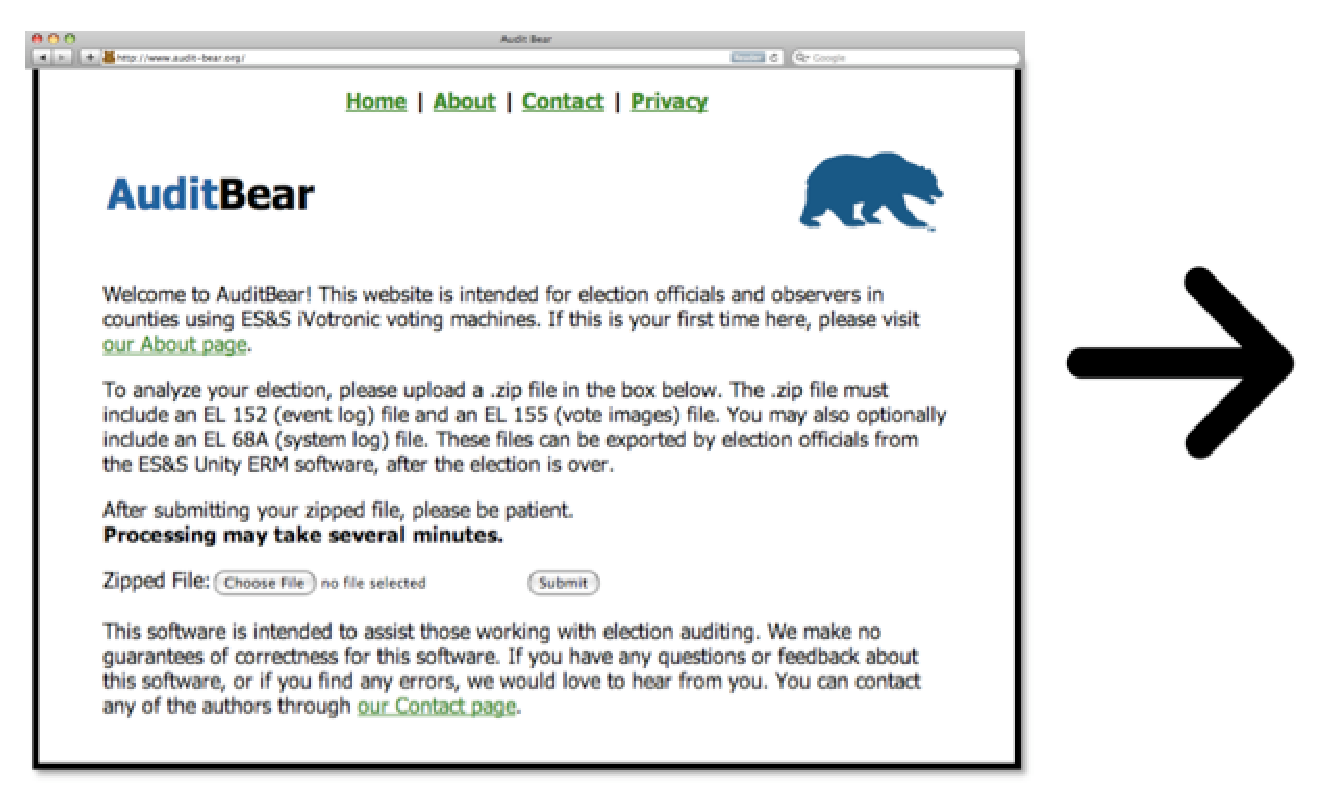
\includegraphics[scale=0.10]{indexpage.eps}
%\end{figure}
%\begin{figure}
%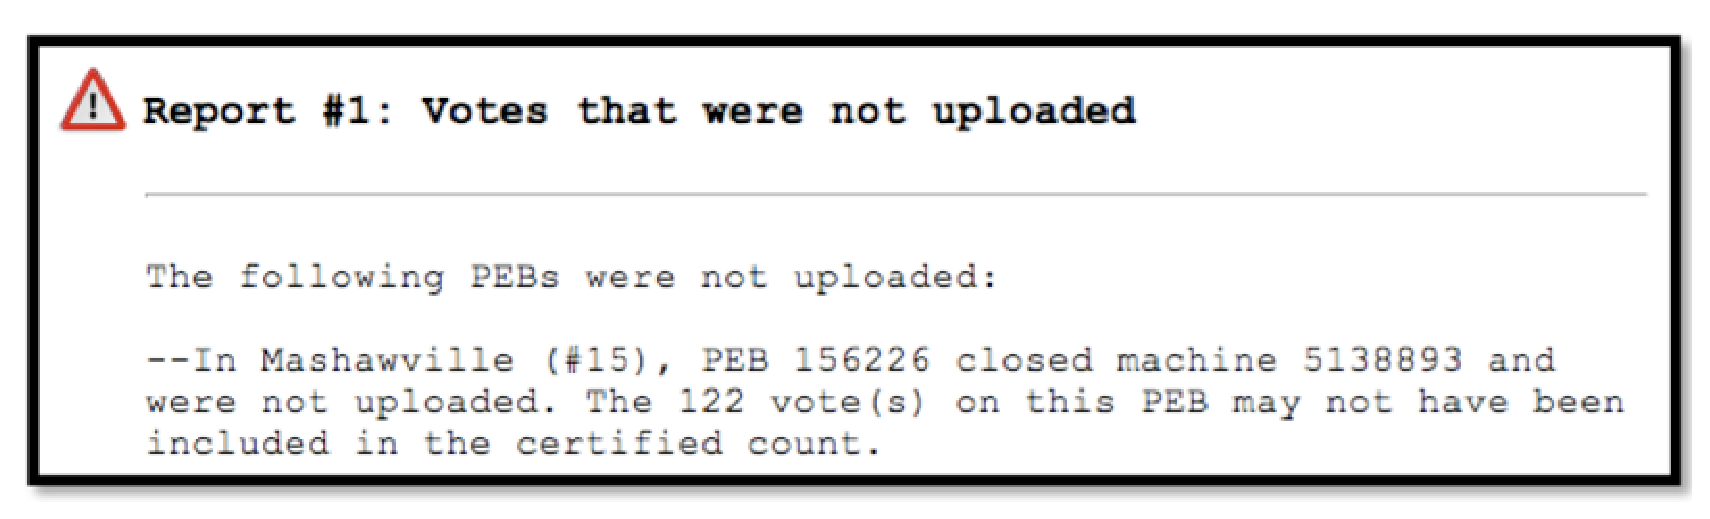
\includegraphics[scale=0.10]{report.eps}
%\end{figure}
